\chapter{Стандарт 802.11 WLAN}

По стандарту 802.11 не обеспечивается отправка пакетов непосредственно на другой
компьютер. Вместо этого, в заголовок пакета помещается адрес желаемой станции
получателя и отправляет пакет в эфир.  Каждый сетевой узел в зоне покрытия
получает все пакеты и использует первый адрес в заголовке 802.11 WLAN MAC для
определения предназначен ли данный пакет данному сетевому узлу. Если пакет
относится к данному сетевому узлу, он записывает его, помещает в память и затем
переходит на следующий слой протокола стека для обработки.  Если сообщение не
было повреждено, то узел обычно отправляет пакет с флагом ACK для подтверждения
этого.

На рисунке~\ref{fig:wlan_diagram} продемонстрирована передача пакетов между
устройствами, устройство А передаёт пакет устройству С. Все устройства в зоне
покрытия получают пакет, который содержит адрес устройства C, но устройства B, D
и E игнорируют данный пакет, когда обнаруживают, что первый адрес в поле
заголовка MAC не совпадает с его собственным адресом. Только устройство С,
обнаружив, что пакет предназначен ему, обрабатывает пакет дальше.

\section{Обзор стандарта 802.11 WLAN}

В 1997 году IEEE приняла 802.11, первый стандарт беспроводного доступа LAN. Это
первый стандарт, предлагающий любую из трёх (взаимно несовместимых) реализаций
физического уровня: инфракрасная (ИК) времяимпульсная модуляция, или
радиочастотные (РЧ) сигналы в диапазоне 2.4 ГГц с использованием
псевдослучайной перестройки рабочей частоты (FHSS) или расширения спектра
методом прямой последовательности (DSSS). ИК метод не был коммерчески
реализован. РЧ версия страдала от низкой скорости передачи (2~МБит/с). С целью
увеличения пропускной способности IEEE создал две рабочие  группы (A и B) для
изучения альтернативных реализация стандарта 802.11. В дальнейшем были созданы
группы G и N [1].

\begin{figure}
    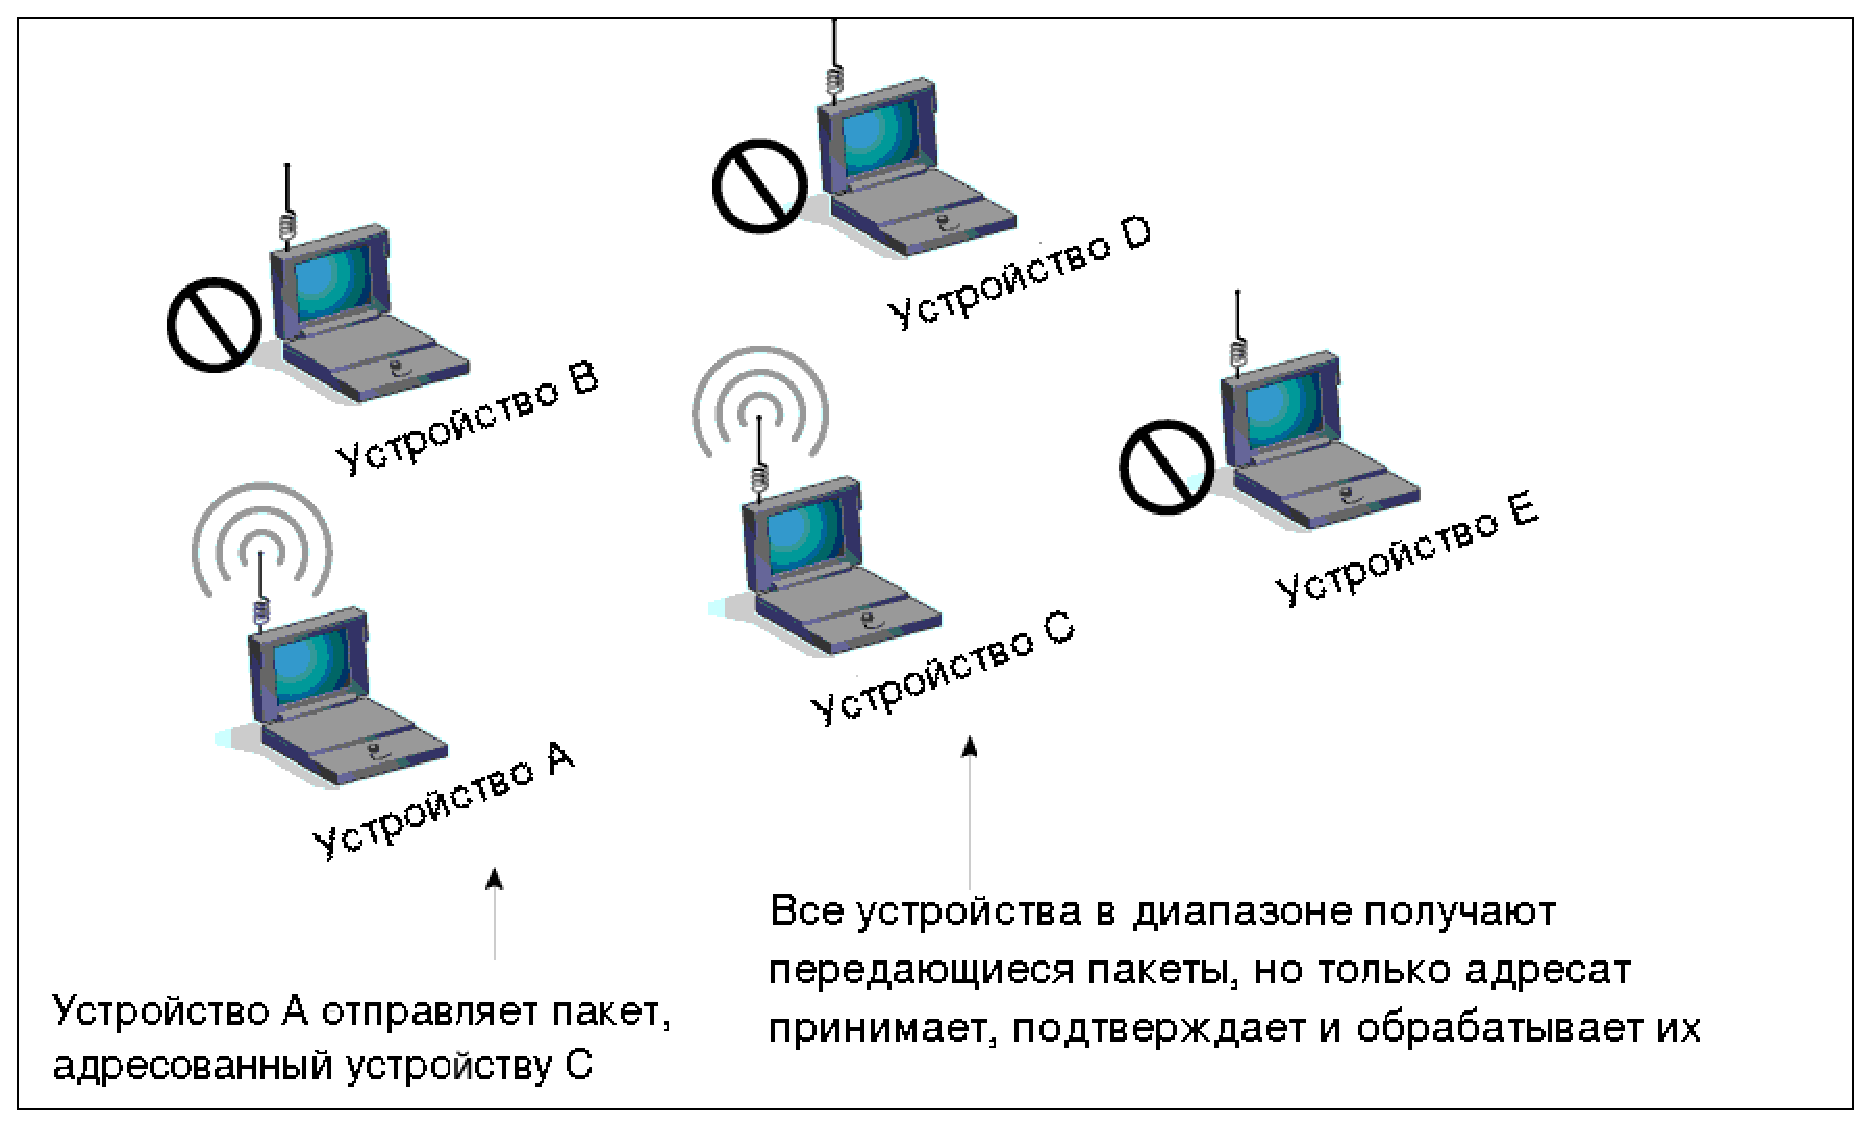
\includegraphics[width=1\textwidth]{graphics/wlan_diagram.eps}
    \caption{Передача пакетов между устройствами}
    \label{fig:wlan_diagram}
\end{figure}

Рабочая группа A исследовала 5.0 ГГц диапазон, используя мультиплексирование с
ортогональным частотным разделением каналов для достижения пропускной
способности около 54 МБит/с. Сложности заключалась в производстве дешёвого
оборудования, работающего на столь больших частотах и в международной
договорённости использования спектра частот, необходимого для стандарта 802.11a.

Европейские инспекторы требуют от 802.11a WLAN устройств поддерживать
дополнительные функции динамического выбора частоты и мощности передачи. Это
поможет предотвратить или снизить уровень потерь между устройствами стандарта
802.11a WLAN и существующими устройствами, использующие 5.0 ГГц диапазон.

Рабочая группа B исследовала более сложные методы DSSS в исходном 2.4 ГГц
диапазоне. Их стандарт 802.11b WLAN был опубликован в сентябре 1999 и позволял
передавать данные на скорости до 11 МБит/с.

Рабочая группа G начала исследование различных методов для дальнейшего
улучшения пропускной способности в 2.4 ГГц диапазоне, который использовался в
стандарте 802.11b. В мае 2001 года федеральное агентство по связи США (FCC) сняла
запрет на использование технологии OFDM в диапазоне 2,4 ГГц. Проект стандарта
IEEE 802.11g был утверждён в октябре 2002 г. Этот стандарт предусматривает
использование диапазона частот 2,4 ГГц, обеспечивая скорость передачи 54 МБит/с
и превосходя, таким образом, стандарт IEEE 802.11b, который обеспечивает
скорость передачи 11 МБит/с. Кроме того, он гарантирует обратную совместимость
со стандартом 802.11b. Обратная совместимость стандарта IEEE 802.11g может быть
реализована в режиме модуляции DSSS, и тогда скорость передачи будет ограничена
одиннадцатью мегабитами в секунду либо в режиме модуляции OFDM, при котором
скорость составляет 54 МБит/с.

Стандарт 802.11n повышает скорость передачи данных практически вчетверо по
сравнению с устройствами стандартов 802.11g (максимальная скорость которых равна
54 МБит/с), при условии использования в режиме 802.11n с другими устройствами
802.11n. Теоретически 802.11n способен обеспечить скорость передачи данных до
600 МБит/с применяя передачу данных сразу по четырём антеннам. По одной антенне,
до 150 МБит/с.

Устройства 802.11n работают в диапазонах 2,4—2,5 или 5,0 ГГц.

Кроме того, устройства 802.11n могут работать в трёх режимах:

\begin{itemize}
    \item наследуемом (Legacy), в котором обеспечивается поддержка устройств 802.11b/g и 802.11a;
    \item смешанном (Mixed), в котором поддерживаются устройства 802.11b/g, 802.11a и 802.11n;
    \item «чистом» режиме — 802.11n (именно в этом режиме и можно воспользоваться
преимуществами повышенной скорости и увеличенной дальностью передачи данных, обеспечиваемыми стандартом 802.11n).
\end{itemize}

Черновую версию стандарта 802.11n (DRAFT 2.0) поддерживают многие современные
сетевые устройства. Итоговая версия стандарта (DRAFT 11.0), которая была принята
11 сентября 2009 года, обеспечивает скорость до 600 МБит/с, Многоканальный
вход/выход, известный, как MIMO и большее покрытие.

Протоколы 802.11 WLAN определяют нижний уровень модели OSI (физический уровень),
и часть следующего, канального, уровня (см. рис.~\ref{fig:osi}). Первоначальная
цель IEEE заключалась в создании набора стандартов, которые могли бы
использовать различные подходы к физическому уровню (различные частоты, методы
кодирования и т.д.), при этом не затрагивая верхние уровни. Они добились успеха,
при этом уровень управления доступом к среде в 802.11a, b, g и n практически
одинаковый.

\begin{figure}
    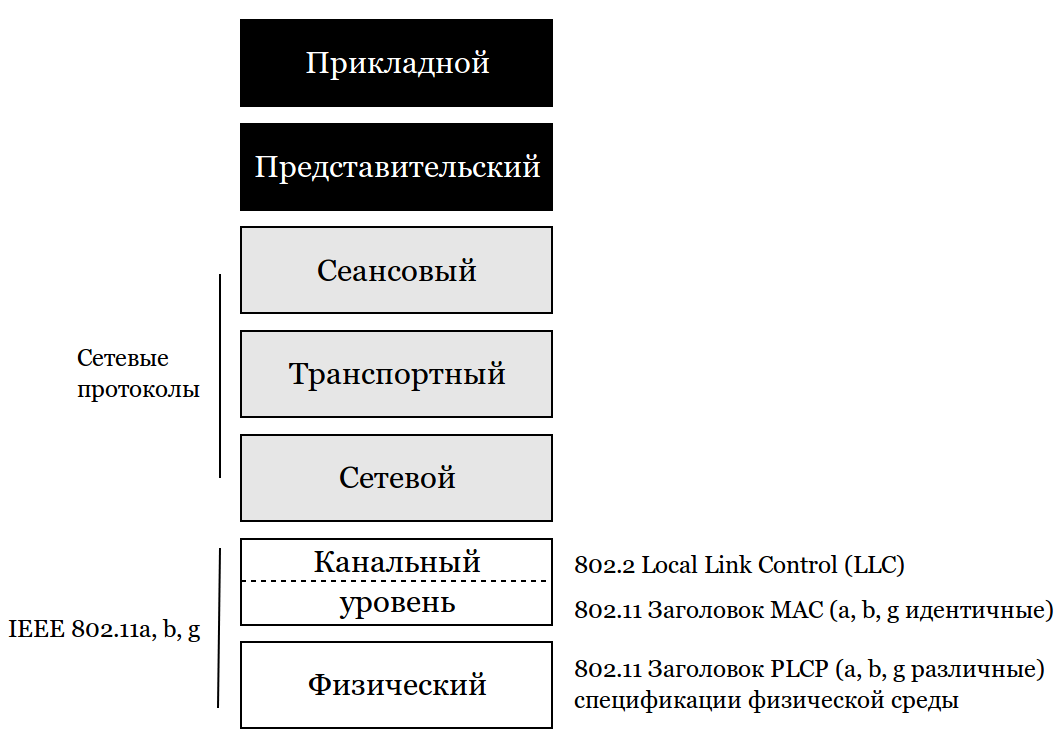
\includegraphics[width=150mm]{graphics/osi.eps}
    \caption{Соответствие 802.11 WLAN модели OSI}
    \label{fig:osi}
\end{figure}

\section{Структура пакета в стандарте 802.11 WLAN}

Каждая часть информации, передаваемая по сети, следуя любому из серии стандартов
IEEE 802, отправляется в так называемом пакете. Пакет является простой порцией
данных, помещённую в одну или более обёртку, которая позволяет идентифицировать
данную порцию данных и правильно её маршрутизировать. Эти обёртки состоят из
заголовков или иногда из заголовков и завершителей. Заголовки являются бинарными
данными, добавленными в начало пакета. Завершители добавляются в конец пакета.
На рисунке~\ref{fig:wifi_packet_theory} представлены блоки, из которых состоит HTTP
пакет, передаваемый по протоколу 802.11 WLAN.

\begin{figure}
    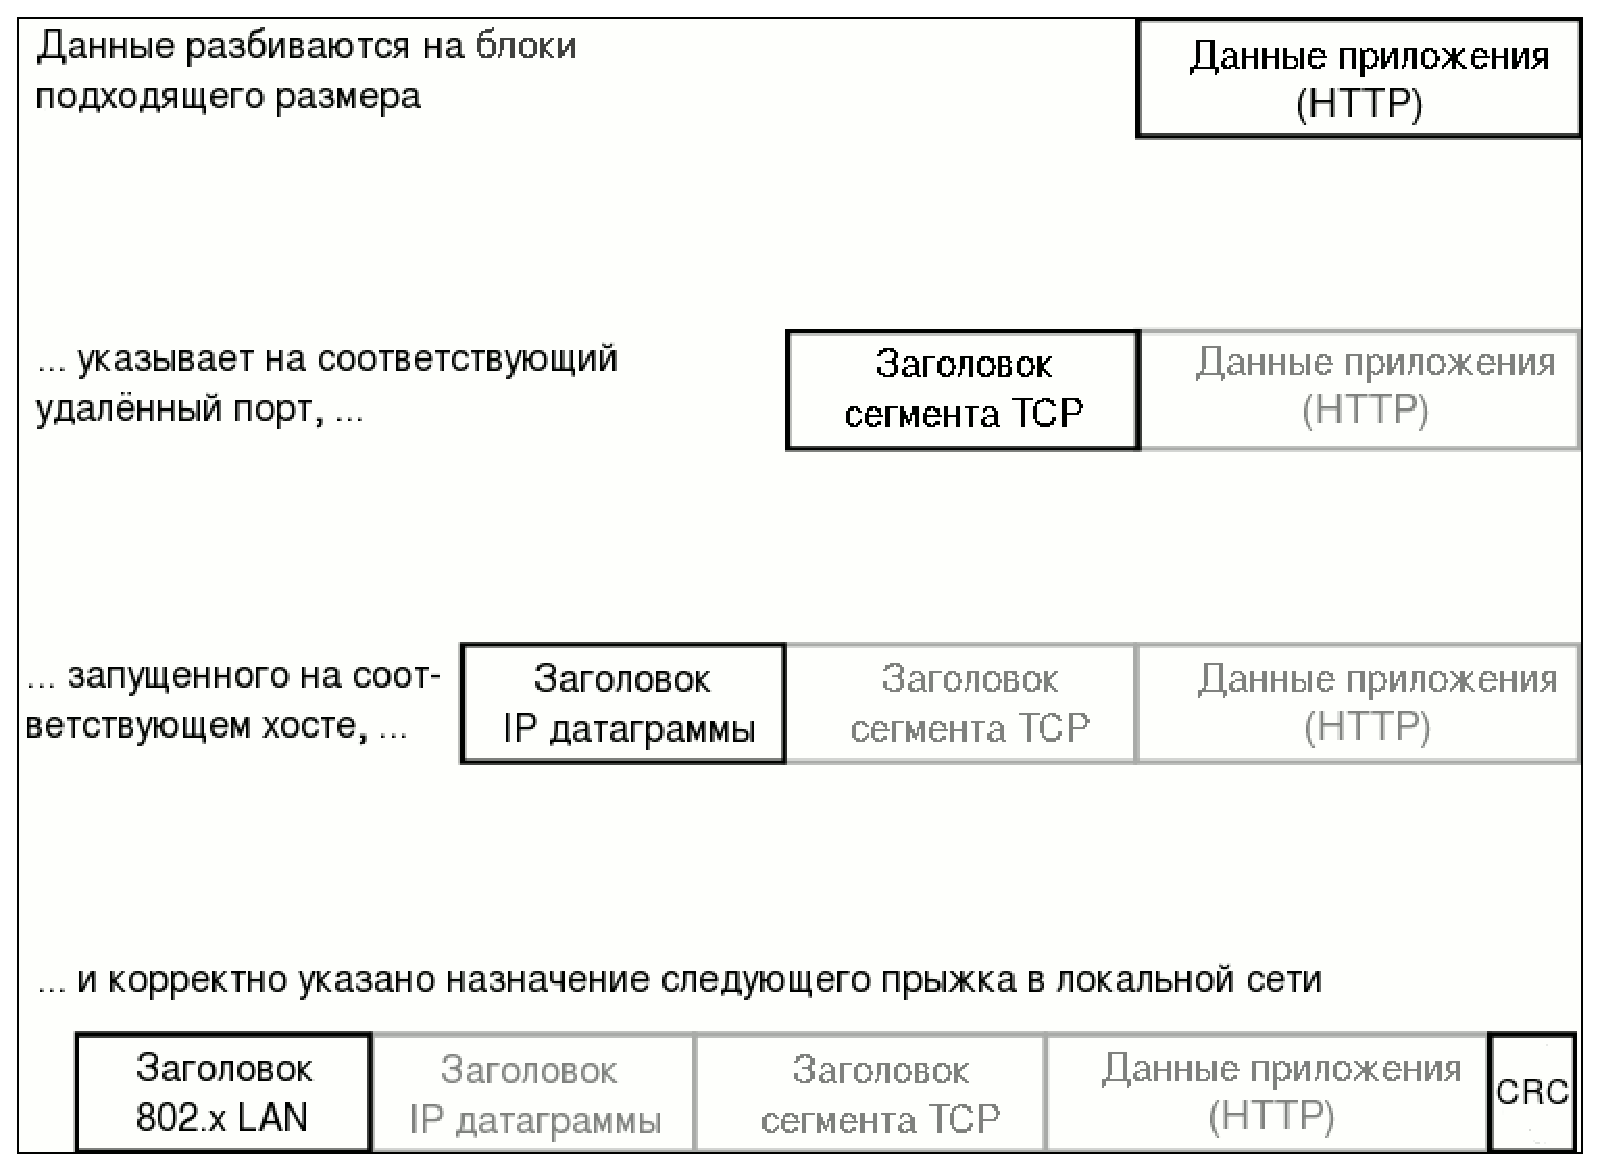
\includegraphics[width=1\textwidth]{graphics/wifi_packet_theory.eps}
    \caption{Структура HTTP пакета, передаваемого по протоколу 802.11}
    \label{fig:wifi_packet_theory}
\end{figure}

Пакеты создаются на машине, которая отправляет информацию. Данные, генерируемые
приложением для отправки, походят в протокол стека, работающие на этой машине.
Протокол стека разбивает данные на порции и оборачивает каждую порцию в одну или
более обёрток, которые позволят пакетам снова собраться в правильном порядка на
стороне получателя. Протокол стека на отправляющей стороне переводит пакеты на
интерфейс сетевой карты.  Сетевое аппаратное обеспечение добавляет свои
собственные обёртки к каждому пакету для направления его к нужному месту
назначения в локальной сети.

Если окончательное место назначения пакета где-то вне локальной сети, то
заголовок, добавленный отправляющим устройством, будет указывать на роутер или
свич при помощи адреса назначения. Роутер будет открывать пакет, вырезать
оригинальную обёртку, считывать окончательный адрес назначения, затем снова
оборачивает пакет, получив новый заголовок пакет отправится на следующий сетевой
узел.

На стороне получателя происходит обратный процесс. Пакет считывается интерфейсом
сетевой карты на получающем устройством, который вырежет сетевой заголовок и
пропустит пакет вверх по соответствующему протоколу сетевого уровня.
Декодированный пакет представлен на рисунке~\ref{fig:wifi_packet_in_sniffer},
где видно какие заголовки прикреплены к HTTP данным. Протокол стека читает и
вырезает свои заголовки и передаёт остальное содержимое пакета вверх к
приложению или процессу, которому он адресован, восстанавливая порции данных в
том порядке, в котором они были отправлены.

Вся функциональность протокола отображается в заголовках пакета. Радиочастотная
технология и мобильные станции накладывают некоторые сложные требования на сети
802.11 WLAN. Эта добавленная сложность находит своё отражение в длинных
заголовках протокола (см. рис.~\ref{fig:wlan_data_packet_structure}) конвергенции
физического уровня (PLCP) а также MAC заголовке.

\begin{figure}
    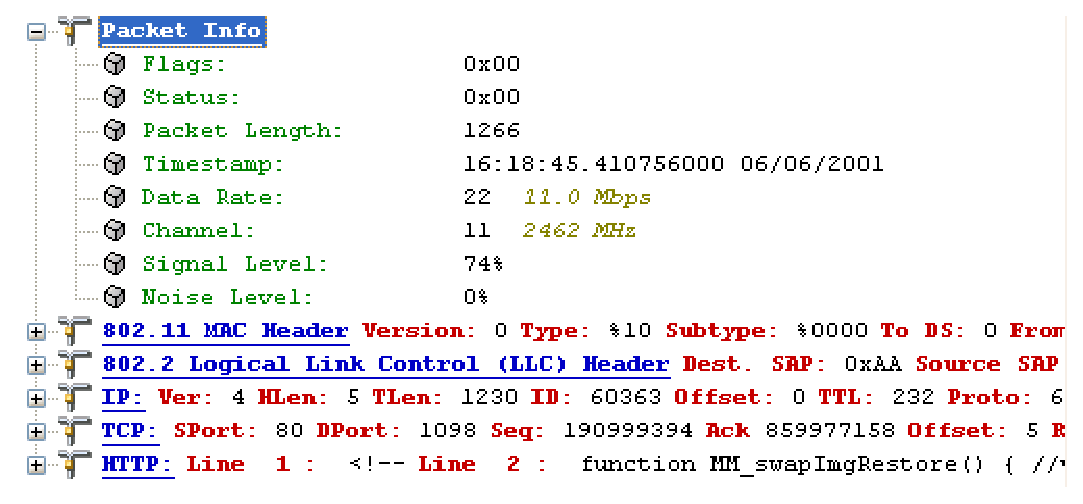
\includegraphics[width=150mm]{graphics/wifi_packet_in_sniffer.eps}
    \caption{Декодированный HTTP пакет, переданный по протоколу 802.11}
    \label{fig:wifi_packet_in_sniffer}
\end{figure}

\begin{figure}
    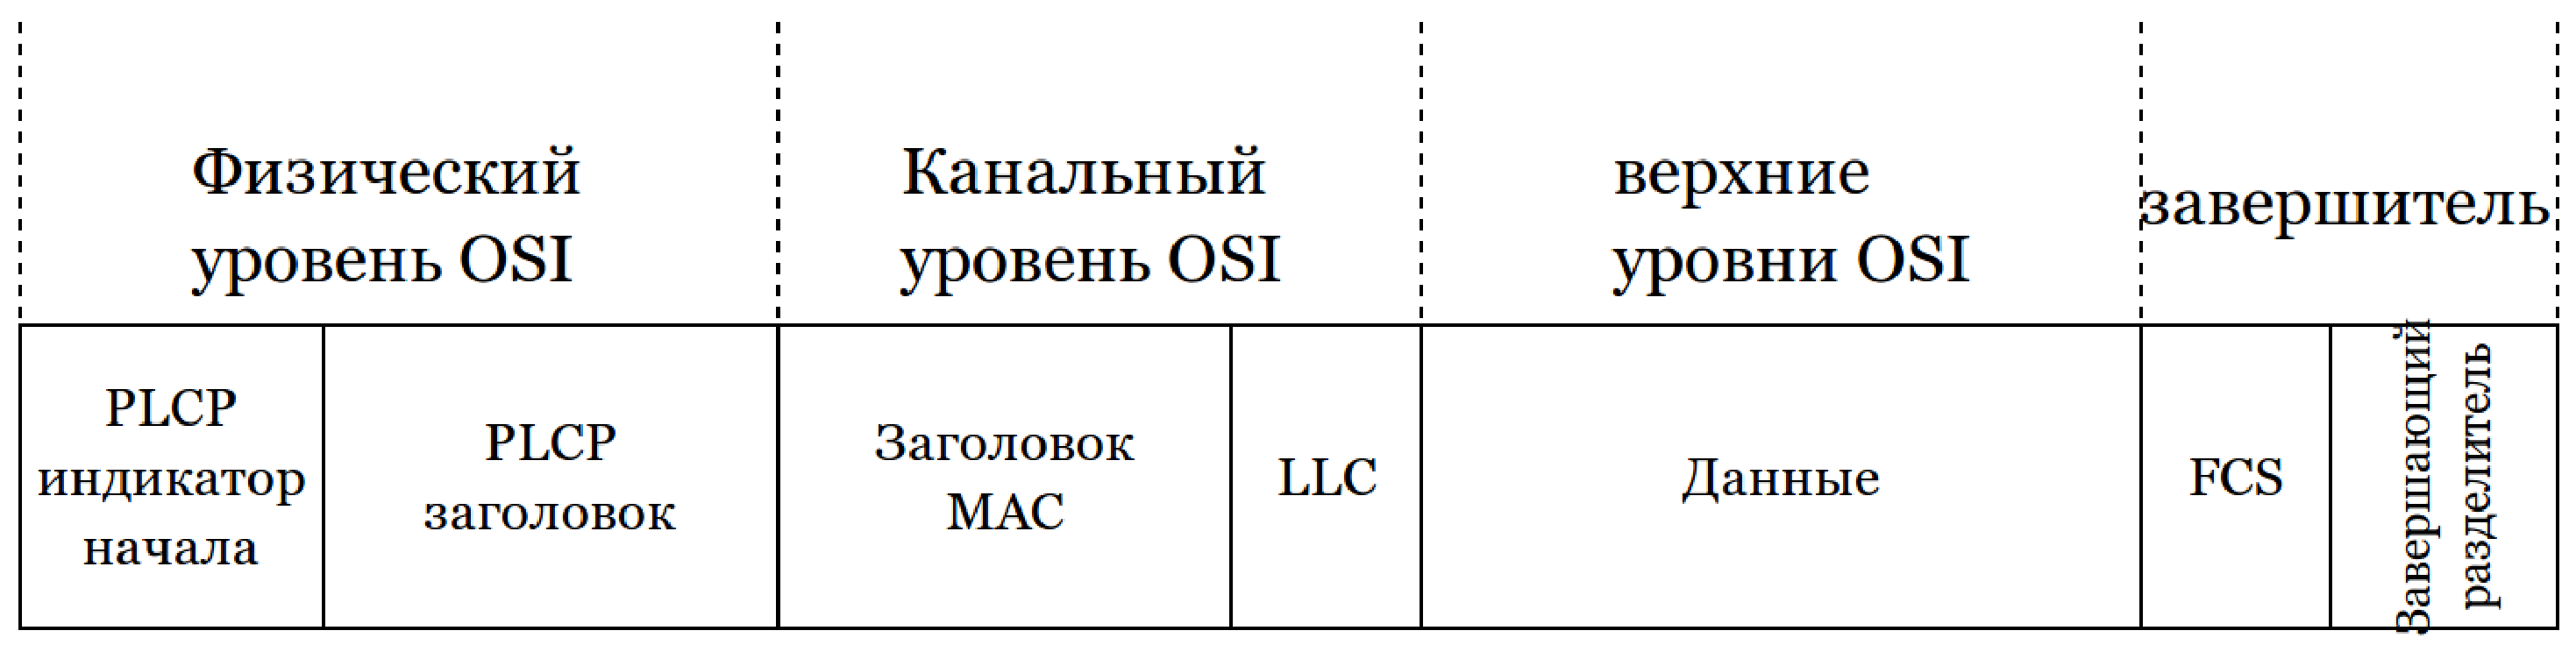
\includegraphics[width=1\textwidth]{graphics/wlan_data_packet_structure.eps}
    \caption{Структура пакета данных 802.11 WLAN}
    \label{fig:wlan_data_packet_structure}
\end{figure}

Так как 802.11 WLAN должны быть в состоянии сформировать и переформировать
список пользователей постоянно и из-за условий радиопередачи, которая может
измениться сама по себе, координация становится большим вопросом для
беспроводных локальных сетей. Кроме того, заголовки обычных WLAN пакетов данных
содержат гораздо больше информации о сетевой топологии и состоянии, чем,
например, заголовки Ethernet пакетов данных (см.
рис.~\ref{fig:compare_mac_wlan_vs_ethernet}).

\section{Аутентификация и конфиденциальность}

Аутентификация ограничивает возможность отправлять и получать информацию по сети.
Конфиденциальность обеспечивает невозможность чтения сетевого трафика
злоумышленником.

\begin{figure}
    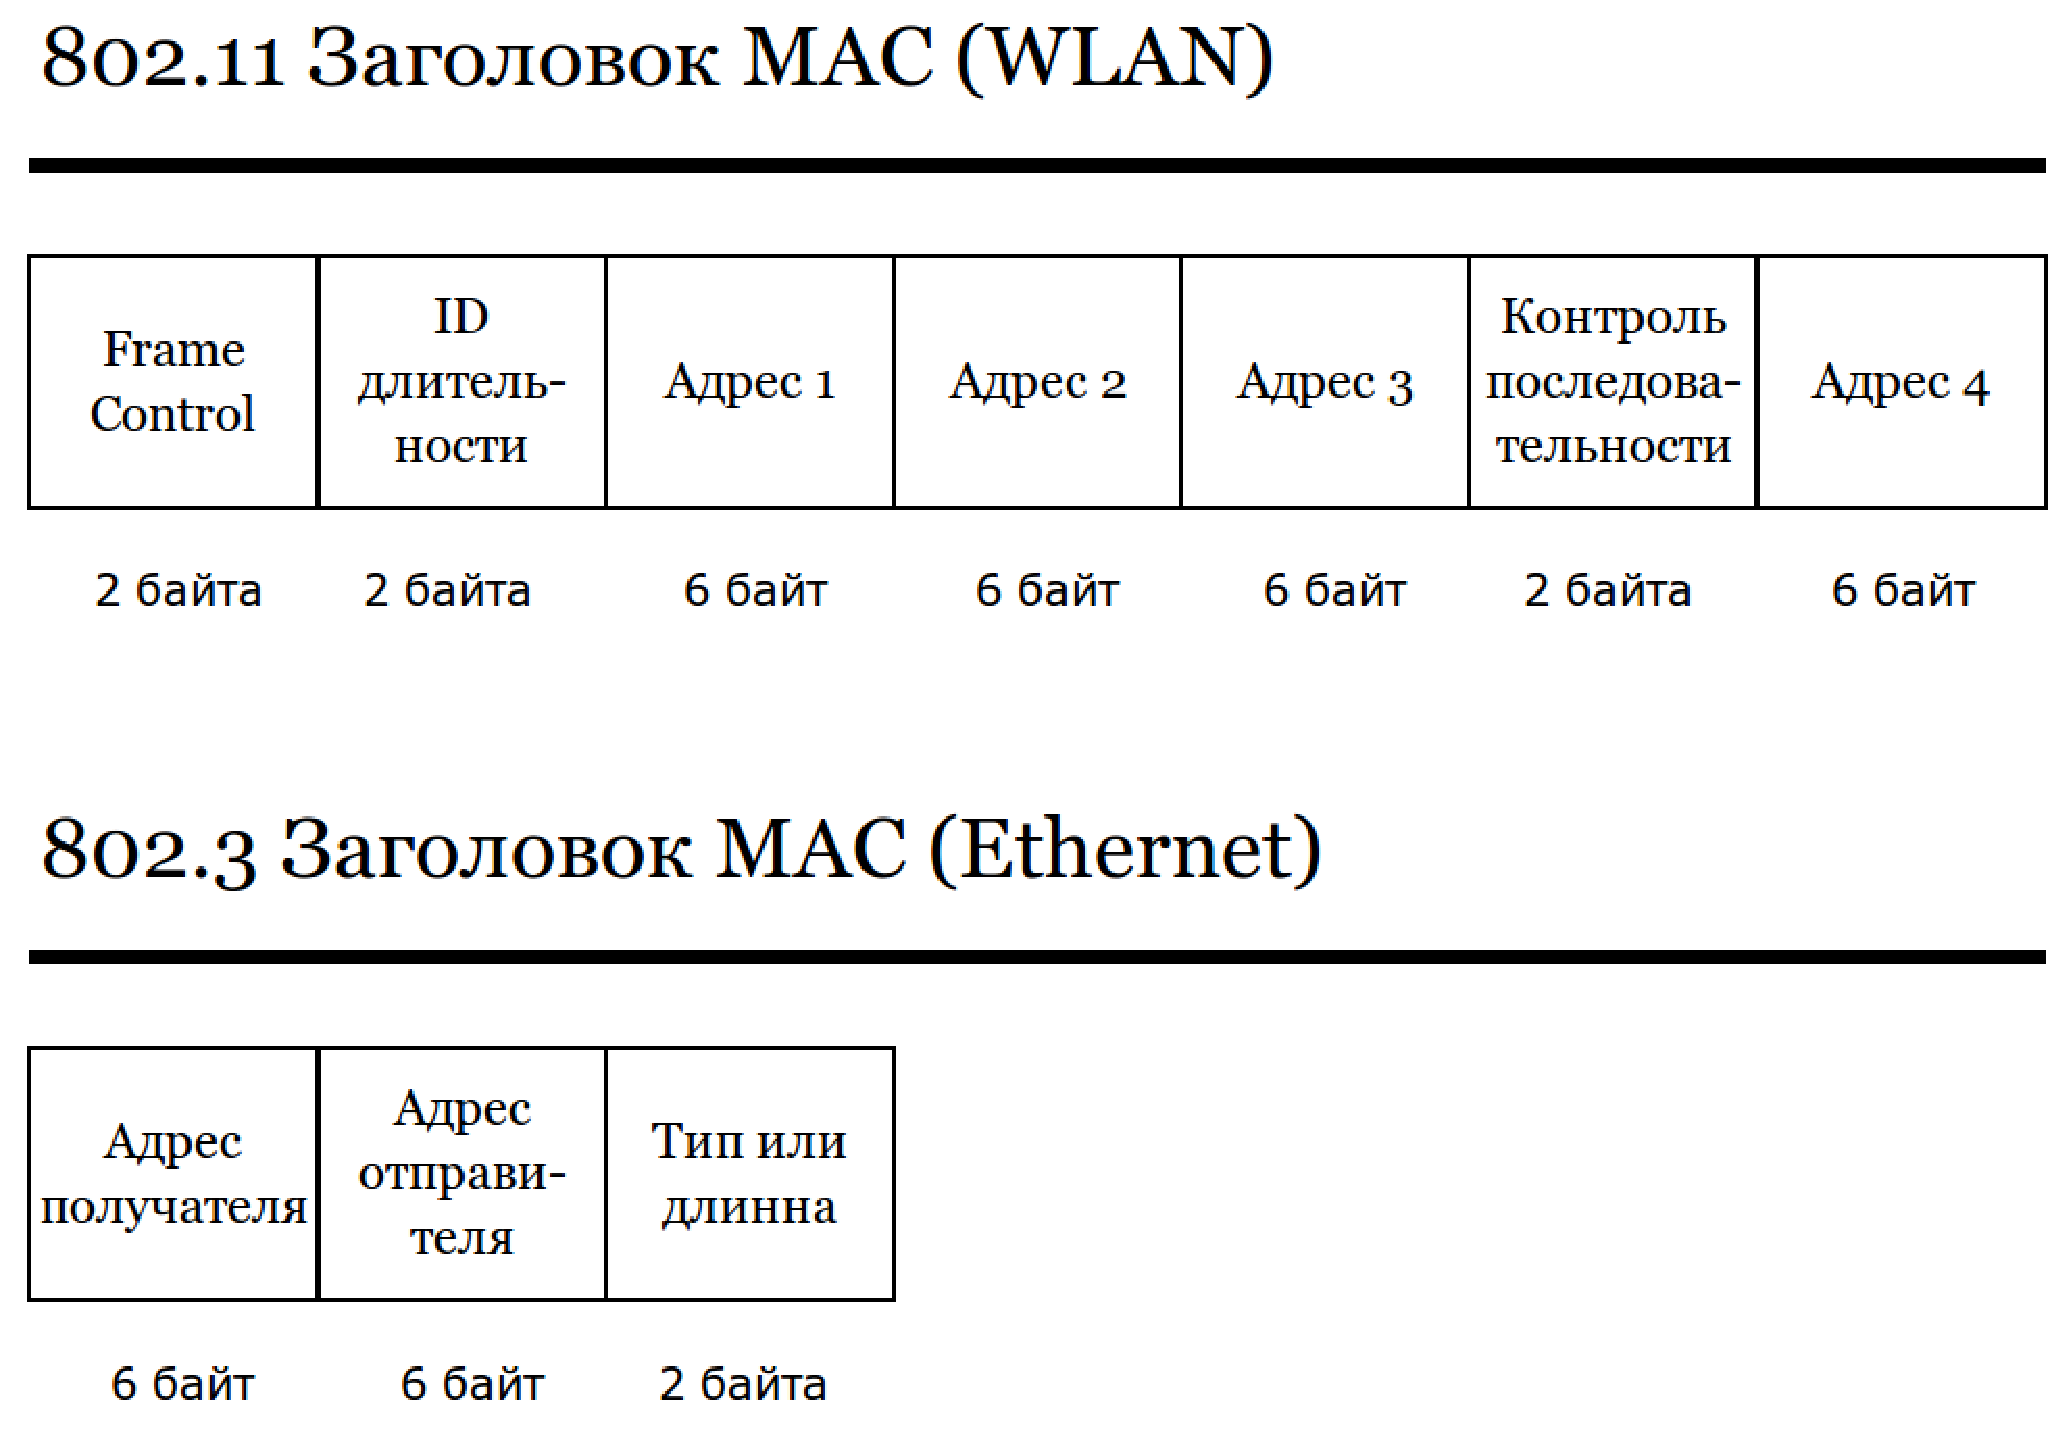
\includegraphics[width=1\textwidth]{graphics/compare_mac_wlan_vs_ethernet.eps}
    \caption{Сравнение MAC заголовков: 802.11 WLAN, 802.3 Ethernet}
    \label{fig:compare_mac_wlan_vs_ethernet}
\end{figure}

Аутентификация может быть открытой или основанной на знании общего ключа. В
любом случае, аутентификация является первым шагом при попытке подключения
устройства к 802.11 беспроводной сети. В случае открытой аутентификации любое
устройство, соответствующее стандарту, будет аутентифицировано. Если
аутентификация основана на общем ключе, то устройство должно подтвердить знание
общего ключа в процессе аутентификации.

WEP --- метод шифрования данных, опционально поддерживающийся протоколами 802.11
WLAN. Метод использует общие ключи и псевдослучайное число в качестве вектора
инициализации для шифрования данных сетевых пакетов. Заголовки 802.11 WLAN не
шифруются.

Целью разработчиков было обеспечение уровня безопасности, в частности защиту от
подслушивания, сравнимый с проводными сетями без шифрования. Прослушивание
проводной сети требует физический доступ к сетевому кабелю или набор сложных
радиопрослушивающих устройств. В то время как для прослушивания трафика 802.11
WLAN достаточно устройства с возможностью слушать определённый канал или
частоту. Все сетевые 802.11 WLAN адаптеры имеют возможность слушать любые
используемые каналы, таким образом вероятность прослушивания довольно велика,
учитывая достаточно большое количество устройств, находящихся в обращении.

Первая WEP спецификация использовала шифрование с ключом длинной 64 бита. В
частности, это было сделано для обеспечения возможности экспорта коммерческих
реализаций за территорию США. В то время только слабые технологии шифрования
могли были экспортироваться. Она предназначена для того, чтобы остановить
случайное подслушивание, но не обеспечивает защиту от целенаправленной атаки.
Некоторые производители сейчас поддерживают длину ключа 64 и 128 бит. Это
увеличивает сложность атаки, но даже ключи длинной 128 бит не обеспечивают
необходимый уровень безопасности.

%\begin{tabular}{ | p{3cm} | p{13cm} |} \caption{Функции протокола } \hline
%\multicolumn{2}{| c |}{Аутентификация / Конфиденциальность} \\ \hline
%\multicolumn{2}{| l |}{Аутентификация - первый шаг этапа присоединения к BSS
%или IBSS. Аутентификация осуществляется обменом управляющих пакетов.} \\ \hline
%authentication ID & Это имя, под которым текущая станция аутентифицировалась
%при вступлении в сеть \\ \hline WEP enabled & Если это поле содержит true,
%тогда данные пакета, но не заголовки WLAN, будут зашифрованы используя WEP \\
%\hline \end{tabular}

% TODO Расписать протокол аутентификации
